\section{LEVEL 2 · Steekproef en populatie}

\begin{missie}
Missie: weet over wie je iets wil zeggen en wie je echt bevraagt. (LPD 11)
\end{missie}

\begin{doel}
\textbf{DOEL} \quad Na dit level kan je:

☐ het verschil uitleggen tussen een \textbf{populatie} ($N$) en een \textbf{steekproef} ($n$);

☐ \textbf{redenen} geven om met een steekproef te werken;

☐ \textbf{steekproefvariabiliteit} herkennen en verklaren;

☐ de drie vormen van statistiek herkennen: \textbf{verzamelende}, \textbf{beschrijvende} en \textbf{verklarende} statistiek.
\end{doel}

\subsection*{Theorie 2.1 · Populatie en steekproef}

\begin{theorie}
\begin{itemize}
\item De \textbf{populatie} is de verzameling van alle mensen, dieren of voorwerpen waarover we informatie willen. Het aantal elementen noemen we de \textbf{populatiegrootte} of populatieomvang: $N$. Dat getal is in de praktijk vaak onbekend.
\item De \textbf{steekproef} is het deel van de populatie dat effectief wordt onderzocht, met als doel betrouwbare informatie te krijgen over de hele populatie. Het aantal elementen is de \textbf{steekproefgrootte} of steekproefomvang: $n$.
\end{itemize}
\end{theorie}

\begin{voorbeeld}
\textbf{Voorbeeld.} Een jeugdhuis heeft 320 ingeschreven jongeren. De werking bevraagt er 60 over hun favoriete activiteit.

Populatie: alle 320 ingeschreven jongeren ($N=320$). Steekproef: de 60 bevraagde jongeren ($n=60$). Variabele: favoriete activiteit (kwalitatief, categorisch niet-geordend).
\end{voorbeeld}

\subsection*{Theorie 2.2 · Waarom een steekproef?}

\begin{theorie}
\begin{itemize}
\item \textbf{Te duur en/of te veel tijd.} Alle 600\,000 Vlaamse leerlingen bevragen zou veel te veel geld en tijd kosten.
\item \textbf{Ethische redenen.} Een nieuw geneesmiddel test je eerst bij een kleine groep, niet meteen bij alle (ernstig zieke) patiënten.
\item \textbf{Het onderzoek vernietigt de populatie.} Als je test bij welke druk een kinderzitje of helm breekt, heb je daarna geen exemplaar meer om te verkopen.
\end{itemize}
\end{theorie}

\subsection*{Theorie 2.3 · Steekproefvariabiliteit}

\begin{theorie}
Verschillende steekproeven uit dezelfde populatie die op dezelfde manier zijn samengesteld, geven vaak \textbf{verschillende resultaten}. Dat noemen we \textbf{steekproefvariabiliteit}. Het is normaal: elke steekproef bestaat uit andere elementen.
\end{theorie}

\begin{voorbeeld}
\textbf{Voorbeeld.} Een school trekt tien keer een steekproef van 30 leerlingen en vraagt hoeveel uur ze per dag naar een scherm kijken. De steekproefgemiddelden (in uur):

\breedtes{9/9/9/9/9/9/9/9/9/9}
\begin{tabular}{cccccccccc}
\hline
1 & 2 & 3 & 4 & 5 & 6 & 7 & 8 & 9 & 10 \\
\hline
3,4 & 3,1 & 3,7 & 3,3 & 3,6 & 3,0 & 3,5 & 3,2 & 3,8 & 3,4 \\
\hline
\end{tabular}

De tien gemiddelden verschillen onderling (van 3,0 tot 3,8 uur), maar liggen in dezelfde buurt. Het gemiddelde van alle tien is 3,4 uur.
\end{voorbeeld}

\subsection*{Theorie 2.4 · De drie vormen van statistiek}

\begin{theorie}
\begin{itemize}
\item \textbf{Verzamelende statistiek}: data verzamelen bij een onderzoeksvraag, bijvoorbeeld via een enquête of experiment.
\item \textbf{Beschrijvende statistiek}: de verzamelde data voorstellen en analyseren met tabellen, grafieken en kengetallen.
\item \textbf{Verklarende statistiek}: de resultaten van de steekproef \emph{veralgemenen} naar de hele populatie.
\end{itemize}
\end{theorie}

\begin{center}
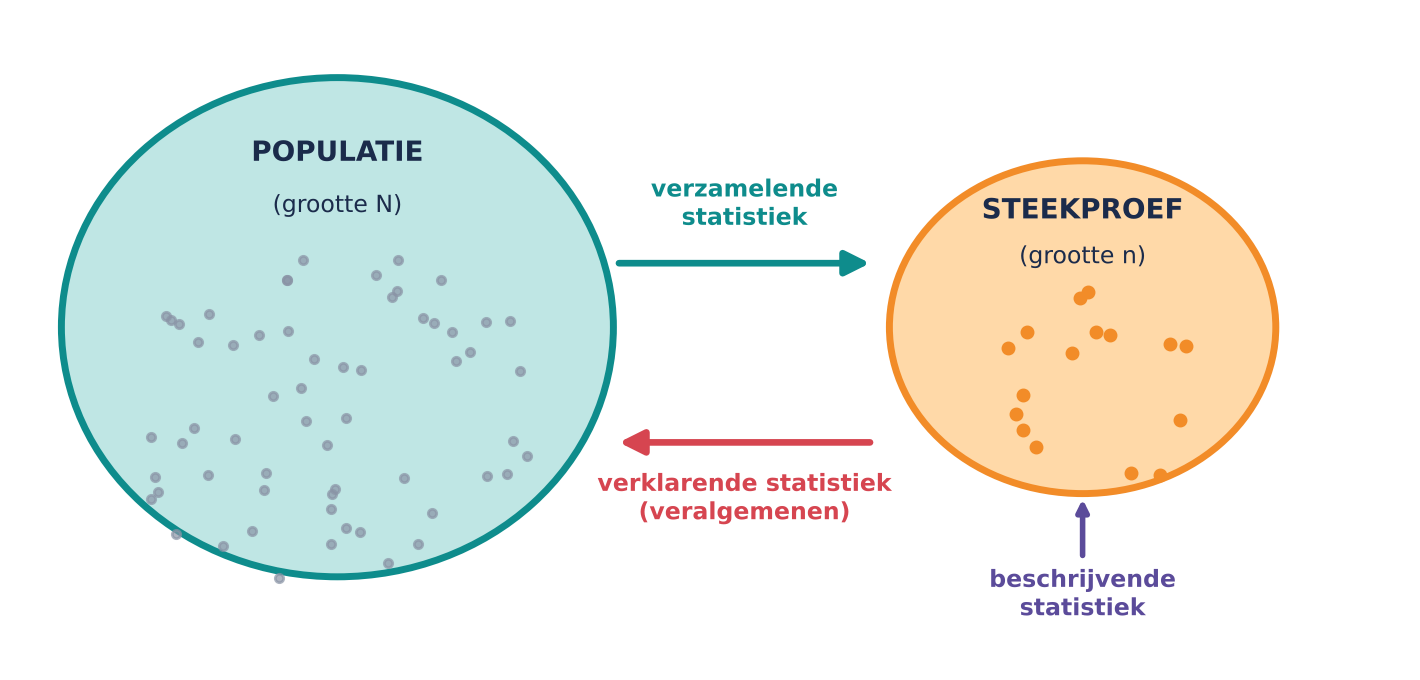
\includegraphics[width=0.85\textwidth]{figuren/d1_vormen.png}
\end{center}

\begin{voorbeeld}
\textbf{Voorbeeld.} Een onderzoeksbureau bevraagt 400 jongeren over hun studentenjob (verzamelend). De antwoorden worden samengevat in een staafdiagram en een gemiddelde (beschrijvend). Op basis daarvan stelt men dat ‘ongeveer een derde van alle Vlaamse jongeren een studentenjob doet om snel geld te verdienen’ (verklarend).
\end{voorbeeld}

\subsection*{Aan de slag}

\subsubsection*{Oefening 2.1 \quad ★☆☆ \quad Invullen}

\textbf{Woordenlijst:} populatie – steekproef – $N$ – $n$ – steekproefvariabiliteit – verklarende.

De \gat{populatie} is de groep waarover we iets willen weten. Het aantal elementen ervan noteren we met \gat{$N$}. Het deel dat we onderzoeken is de \gat{steekproef}, met omvang \gat{$n$}. Doordat elke steekproef uit andere elementen bestaat, krijg je telkens andere resultaten: dat is \gat{steekproefvariabiliteit}. Het veralgemenen van de resultaten naar de hele populatie is \gat{verklarende} statistiek.

\subsubsection*{Oefening 2.2 \quad ★★☆ \quad Koppel: vraag en antwoord}

Een school met 978 leerlingen laat een nieuwe huisstijl ontwerpen. Een mini-enquête wordt afgenomen bij 220 leerlingen met de vraag: ‘Hoe tevreden ben je? (zeer ontevreden – ontevreden – neutraal – tevreden – zeer tevreden)’. Koppel elke vraag (A – F) aan het juiste antwoord (1 – 6).

\breedtes{50/50}
\begin{tabular}{ll}
\hline
Vraag & Antwoord \\
\hline
A. Hoeveel leerlingen werden bevraagd? & 1. De populatieomvang is 978. \\
B. Wie wordt er bevraagd? & 2. Categorisch geordend. \\
C. Over welke groep wil men iets besluiten? & 3. De steekproefomvang is 220. \\
D. Wat is $N$? & 4. Alle 978 leerlingen van de school. \\
E. Welk soort data werd verzameld? & 5. Kwalitatief. \\
F. Welk soort variabele werd onderzocht? & 6. De 220 leerlingen die de enquête invulden. \\
\hline
\end{tabular}

A – \_\_ \quad B – \_\_ \quad C – \_\_ \quad D – \_\_ \quad E – \_\_ \quad F – \_\_

\begin{oplossing}
\textbf{Oplossing 2.2} \quad A – 3 \quad B – 6 \quad C – 4 \quad D – 1 \quad E – 2 \quad F – 5
\end{oplossing}

\subsubsection*{Oefening 2.3 \quad ★★☆ \quad Waarom een steekproef?}

Noteer bij elke situatie de belangrijkste reden om met een steekproef te werken.

\textbf{a)} Een fabrikant test hoeveel druk een kinderstoel kan weerstaan voor die breekt. \lijn

\textbf{b)} Een onderzoeker wil de mentale gezondheid van alle 11 miljoen Belgen kennen. \lijn

\textbf{c)} Een nieuw vaccin voor baby’s wordt eerst bij een kleine groep getest. \lijn

\begin{oplossing}
\textbf{Oplossing 2.3} \quad a) Het onderzoek vernietigt de populatie (de stoelen zijn stuk). b) Te duur en te veel tijd. c) Ethische redenen: je wil niet meteen alle baby’s blootstellen aan een nog niet geteste behandeling.
\end{oplossing}

\subsubsection*{Oefening 2.4 \quad ★★☆ \quad Steekproefvariabiliteit}

Bekijk de tien steekproefgemiddelden in het voorbeeld van theorie 2.3.

\textbf{a)} Tussen welke twee waarden liggen alle gemiddelden? Hoe groot is het verschil? \lijn

\textbf{b)} Waarom zijn de tien gemiddelden niet gelijk, terwijl alle steekproeven op dezelfde manier zijn getrokken? \lijn

\textbf{c)} De school trekt nu steekproeven van 300 in plaats van 30 leerlingen. Wat verwacht je over de gemiddelden? \lijn

\begin{oplossing}
\textbf{Oplossing 2.4} \quad a) Tussen 3,0 en 3,8 uur; verschil 0,8 uur. b) Elke steekproef bevat andere leerlingen: steekproefvariabiliteit. c) De gemiddelden liggen dichter bij elkaar (en bij het populatiegemiddelde): grotere representatieve steekproeven geven een kleinere afwijking.
\end{oplossing}

\subsubsection*{Oefening 2.5 \quad ★★☆ \quad Koppel: welke vorm van statistiek?}

Schrijf V (verzamelend), B (beschrijvend) of K (verklarend) bij elke situatie.

\breedtes{80/20}
\begin{tabular}{ll}
\hline
Situatie & V / B / K \\
\hline
a) Een zorgorganisatie laat 150 medewerkers een vragenlijst over werkdruk invullen. & \\
b) De resultaten worden samengevat in een staafdiagram en een gemiddelde. & \\
c) Men besluit: ‘Zorgverleners in Vlaanderen ervaren gemiddeld een hoge werkdruk.’ & \\
d) Een leerkracht noteert in Excel de scores van zijn 24 leerlingen en berekent het klasgemiddelde. & \\
\hline
\end{tabular}

\begin{oplossing}
\textbf{Oplossing 2.5} \quad a) V \quad b) B \quad c) K \quad d) B
\end{oplossing}

\subsubsection*{Oefening 2.6 \quad ★★★ \quad Context: een krantenkop onder de loep}

Een krant schrijft: ‘Vlamingen slapen te weinig: slechts 4 op 10 haalt zeven uur slaap.’ Het onderzoek gebeurde bij 1\,200 Vlamingen.

\textbf{a)} Is het realistisch dat alle Vlamingen werden bevraagd? Geef twee redenen. \lijn

\textbf{b)} Een tweede onderzoeksbureau voert hetzelfde onderzoek uit bij 1\,200 andere Vlamingen. Is het percentage dan exact 40 \%? Verklaar. \lijn

\textbf{c)} Noteer de populatie, de steekproef, $N$ (bekend of niet?) en $n$. \lijn

\begin{oplossing}
\textbf{Oplossing 2.6} \quad a) Nee: te duur en te veel tijd; praktisch onmogelijk. b) Niet noodzakelijk: andere personen, dus een ander resultaat (steekproefvariabiliteit). c) Populatie: alle Vlamingen; steekproef: de 1\,200 bevraagde Vlamingen; $N$ is niet exact gekend (ongeveer 6,7 miljoen, wisselt); $n=1200$.
\end{oplossing}

\subsection*{Foutjager}

\textbf{1.} Jana: ‘Ik bevroeg 40 van de 200 leden: 25 \% zegt ja. Dus precies 25 \% van alle leden zegt ja.’ \lijn

\textbf{2.} Ruben: ‘Mijn steekproef is de volledige populatie, want ze is groot.’ \lijn

\begin{oplossing}
\textbf{Oplossing Foutjager} \quad 1. Het steekproefresultaat is slechts een schatting; door steekproefvariabiliteit kan het populatieaandeel licht afwijken. 2. Een steekproef is een deel van de populatie; ook een grote steekproef is niet de hele populatie.
\end{oplossing}

\subsection*{CHECK · Level 2}

\textbf{1.} (2 p) Een school met 600 leerlingen bevraagt 80 leerlingen. Noteer $N$, $n$ en de steekproef. \lijn

\textbf{2.} (3 p) Noem drie redenen om met een steekproef te werken. \lijn

\textbf{3.} (2 p) Verklaar steekproefvariabiliteit met een voorbeeld. \lijn

\textbf{4.} (2 p) Wat is het verschil tussen beschrijvende en verklarende statistiek? \lijn

\begin{doel}
\textbf{Score:} \_\_\_ / 9 \quad ☐ behaald (vanaf 6 / 9) \quad ☐ nog even oefenen
\end{doel}

\begin{oplossing}
\textbf{Oplossing CHECK 2} \quad 1. $N=600$; $n=80$; de steekproef is de groep van 80 bevraagde leerlingen. 2. Te duur/te veel tijd; ethische redenen; het onderzoek vernietigt de populatie. 3. Twee steekproeven van 30 leerlingen geven bijvoorbeeld gemiddelden van 3,1 en 3,6 uur, omdat het andere leerlingen zijn. 4. Beschrijvend: de data van de steekproef voorstellen en samenvatten. Verklarend: de resultaten veralgemenen naar de populatie.
\end{oplossing}
